\documentclass[11pt]{article}
\usepackage[margin=1in]{geometry}
\usepackage[pdftex]{graphicx}
\usepackage{amsmath,amssymb,amsthm}
\usepackage{custom}
\usepackage{tikz}
\usetikzlibrary{calc}

% color boxes
\usepackage[many]{tcolorbox}
\tcbuselibrary{theorems}
\newtcbtheorem{psexample}{Example}{colback=green!10,colframe=green!40!black,fonttitle=\bfseries,breakable,enhanced}{ex}
\newtcbtheorem{psidea}{Idea}{colback=blue!10,colframe=blue!40!black,fonttitle=\bfseries,breakable,enhanced}{id}
\newtcbtheorem{psremark}{Remark}{colback=purple!10,colframe=purple!40!black,fonttitle=\bfseries,breakable,enhanced}{rm}
\newtcbtheorem{pssolution}{Solution}{colback=orange!10,colframe=orange!40!black,fonttitle=\bfseries,breakable,enhanced}{sn}

\newtheorem{pproblem}{Problem}

% headers and footers
\usepackage{fancyhdr}
\pagestyle{fancy}
\lhead{Rolling Without Slipping}
\chead{}
\rhead{Mechanics}
\lfoot{}
\cfoot{\thepage}
\rfoot{}
\renewcommand{\headrulewidth}{0.4pt}
\setlength{\headheight}{14pt}

\newcommand{\psettitle}[1]{
    \begin{center}
    \huge \textbf{#1}
    \end{center}
}

\linespread{1.03}
\setlength{\parindent}{0.2in}

\begin{document}

\psettitle{Rolling Without Slipping}
\begin{center}
\large Forces and torques vs.\ energy and kinematics --- two roads to the same answer
\end{center}

\section*{Key Facts}

\begin{psidea}{The four things you need to know}{}
\begin{itemize}
\item \textbf{Rolling without slipping} means the contact point is instantaneously at
rest. This forces the center's speed and the spin rate to move in lockstep:
\[
v = \omega r \qquad\text{and, differentiating,}\qquad a = \alpha r.
\]
\item The force that enforces this is \textbf{static} friction, not kinetic friction.
Static friction can point either way and take any magnitude up to $\mu_s N$ --- it is
not automatically at its maximum value. Its job is to supply whatever torque is needed
to keep $v = \omega r$ true.
\item Because the contact point isn't moving, static friction does \textbf{zero work}.
So even though friction is acting, mechanical energy is still conserved --- you can use
energy methods freely.
\item Without friction, a round object released on an incline would slide but never
spin: friction is the \emph{only} thing that can torque it up.
\end{itemize}
\end{psidea}

\section*{The Object: $I = kmr^2$}

Consider a sphere of mass $m$ and radius $r$ whose density depends only on the distance
from its center --- \textbf{spherically symmetric}, but not necessarily uniform (think of
a planet with a dense core, or a ball with an off-brand filling). Symmetry guarantees
that the moment of inertia about \emph{any} axis through the center is the same single
number, so we can always write it as
\[
\boxed{\,I = k\,m r^2\,}
\]
for some dimensionless number $k$ that depends on how the mass is arranged inside,
but not on which diameter happens to be the rolling axis. That is what makes the
problems below solvable without ever knowing the details of the internal structure ---
$k$ is all that matters.

\begin{psremark*}{}{}
For reference, here is $k$ for a few standard shapes (radius $r$, axis through the
center):
\begin{center}
\begin{tabular}{lc}
\textbf{Shape} & $\boldsymbol{k}$ \\
\hline
Hoop / thin ring (mass all at the rim) & $1$ \\
Solid uniform cylinder or disk & $1/2$ \\
Solid uniform sphere & $2/5$ \\
Thin uniform spherical shell & $2/3$ \\
\end{tabular}
\end{center}
You would find these with calculus, by chopping the shape into thin rings or shells and
adding up $I = \int r_\perp^2\, dm$ for each piece. \textbf{That derivation is optional
--- you are not being asked to do it here.} Just take these four values as known
reference points.

One more fact worth knowing: for a filled ball whose density depends only on distance
from the center (exactly our setup), $k$ can range from $0$ (all the mass squeezed to
the very center) up to a maximum of $2/3$ (all the mass pushed out into a thin shell at
the surface) --- a uniform solid sphere's $2/5$ sits right in between. Keep that in mind
in Problem~\ref{prob:cases}: some values of $k$ we test there are useful mathematical
extremes rather than things an actual sphere of this kind could achieve.
\end{psremark*}

\begin{center}
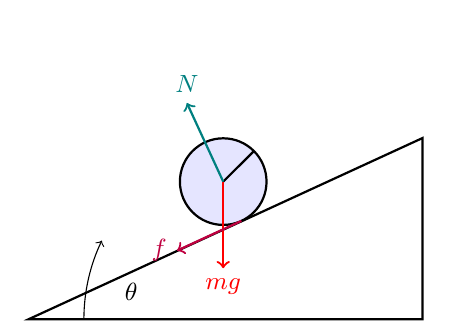
\begin{tikzpicture}[scale=1]
\coordinate (A) at (0,0);
\coordinate (B) at (5,0);
\coordinate (C) at (5,2.3);
\draw[thick] (A) -- (B) -- (C) -- cycle;
\draw[thick] (A) -- (B);
\node[below] at (2.5,0) {};
\draw[->] (0.7,0) arc (180:154.3:2.3) node[midway, below] {};
\node at (1.3,0.35) {\small $\theta$};

% ball on the incline
\pgfmathsetmacro{\thetadeg}{24.8}
\coordinate (P) at (2.7,{2.7*tan(24.8)});
\coordinate (Ctr) at ($(P)+(90+\thetadeg:0.55)$);
\draw[thick, fill=blue!10] (Ctr) circle (0.55);
\draw[thick] (Ctr) -- ($(Ctr)+(20+\thetadeg:0.55)$);

% force arrows
\draw[->, thick, red] (Ctr) -- ++(-90:1.1) node[below] {\small $mg$};
\draw[->, thick, teal] (Ctr) -- ++({90+\thetadeg}:1.1) node[above] {\small $N$};
\draw[->, thick, purple] (P) -- ++({180+\thetadeg}:0.9) node[left] {\small $f$};
\end{tikzpicture}
\end{center}

\section*{Setting Up the Incline}

A sphere of mass $m$, radius $r$, and $I = kmr^2$ is released from rest at the top of an
incline making angle $\theta$ with the horizontal, and rolls down without slipping.
Static friction $f$ (magnitude unknown, direction up the incline) acts at the contact
point, along with gravity $mg$ and the normal force $N$.

\begin{pproblem}[Forces and torques] \label{prob:forces}
Write Newton's second law along the incline and the torque equation about the sphere's
center. Use the rolling constraint to eliminate $\omega$ and $f$, and solve for the
linear acceleration $a$ down the incline in terms of $g$, $\theta$, and $k$.
\end{pproblem}

\begin{pproblem}[Energy and kinematics] \label{prob:energy}
Now forget forces. The incline has length $L$ measured along the slope. Using
conservation of energy, find the sphere's speed $v$ at the bottom, starting from rest at
the top. Then, treating the acceleration as constant, use kinematics to turn that speed
into an acceleration $a$. Confirm you get the same formula as in
Problem~\ref{prob:forces}.
\end{pproblem}

\begin{pproblem}[Testing special cases] \label{prob:cases}
Plug $k = 0$, $k = 1$, and $k \to \infty$ into your formula for $a$. For each case,
state in words what physical situation that value of $k$ describes, and explain in a
sentence or two why the resulting acceleration matches (or doesn't match) your
intuition.
\end{pproblem}

\begin{pproblem}[Optional: how much friction does it take?] \label{prob:friction}
Rolling without slipping only works if the required friction force doesn't exceed what
static friction can supply, $f \le \mu_s N$. Using your result for $f$ from
Problem~\ref{prob:forces} (and $N$ from the perpendicular direction), find the
\emph{minimum} coefficient of static friction $\mu_{\min}(k,\theta)$ needed for the
sphere to roll without slipping, rather than skid. This part is optional --- attempt it
if you want an extra challenge.
\end{pproblem}

\newpage
\section*{Solutions}

\begin{pssolution}{Problem~\ref{prob:forces}}{}
Take down-the-incline as positive. Along the incline,
\[
mg\sin\theta - f = ma. \tag{1}
\]
Gravity acts at the center (no torque about the center) and the normal force's line of
action passes through the center too, so only friction contributes a torque about the
center:
\[
fr = I\alpha = (kmr^2)\alpha. \tag{2}
\]
Rolling without slipping gives $\alpha = a/r$. Substituting into (2):
\[
fr = kmr^2 \cdot \frac{a}{r} \;\Longrightarrow\; f = kma.
\]
Substituting into (1):
\[
mg\sin\theta - kma = ma \;\Longrightarrow\; g\sin\theta = a(1+k)
\]
\[
\boxed{a = \frac{g\sin\theta}{1+k}}
\]
\end{pssolution}

\begin{pssolution}{Problem~\ref{prob:energy}}{}
Dropping height $h = L\sin\theta$, energy conservation (friction does no work, since the
contact point doesn't move) gives
\[
mgh = \tfrac12 mv^2 + \tfrac12 I\omega^2 = \tfrac12 mv^2 + \tfrac12(kmr^2)\left(\frac{v}{r}\right)^2
= \tfrac12 mv^2(1+k).
\]
So
\[
v^2 = \frac{2gh}{1+k} = \frac{2gL\sin\theta}{1+k}.
\]
For constant acceleration from rest over a distance $L$, kinematics gives $v^2 = 2aL$, so
\[
a = \frac{v^2}{2L} = \frac{1}{2L}\cdot\frac{2gL\sin\theta}{1+k} = \frac{g\sin\theta}{1+k},
\]
the same result as Problem~\ref{prob:forces}, as it should be --- these are two
descriptions of the same motion.
\end{pssolution}

\begin{pssolution}{Problem~\ref{prob:cases}}{}
\begin{subpart}
\item $\boldsymbol{k=0}$: $\;a = g\sin\theta$, the same as a block sliding down a
\emph{frictionless} incline. This makes sense: $k=0$ means all the mass sits right at
the center, so it costs nothing to spin the sphere up. In fact $f = kma = 0$ here --- no
friction force is actually needed, so the sphere behaves exactly like frictionless
sliding even though friction is available.

\item $\boldsymbol{k=1}$: $\;a = \tfrac12 g\sin\theta$, exactly half the frictionless
value. At $k=1$ the rotational kinetic energy $\tfrac12 I\omega^2$ equals the
translational kinetic energy $\tfrac12 mv^2$ at every instant, so exactly half of the
released gravitational energy goes into spin and half into forward motion --- hence half
the acceleration. (A hoop has $k=1$ exactly. As noted above, an actual filled sphere of
this kind can't reach $k=1$ --- its ceiling is $k=2/3$ --- so think of this case as
``what a hoop does,'' a useful comparison rather than a literal sphere.)

\item $\boldsymbol{k\to\infty}$: $\;a \to 0$. As $k$ grows, more and more of the released
energy is forced into spinning the object rather than moving it forward, so in the limit
essentially none of it is left for translation and the sphere just sits there rolling in
place with (in principle) zero forward acceleration. This case is a pure mathematical
extreme --- no real sphere of this kind reaches anywhere near it, since $k$ tops out at
$2/3$ --- but it is a good stress test of the formula's behavior.
\end{subpart}
\end{pssolution}

\begin{pssolution}{Problem~\ref{prob:friction}}{}
From Problem~\ref{prob:forces}, $f = kma = \dfrac{kmg\sin\theta}{1+k}$. Perpendicular to
the incline there is no acceleration, so $N = mg\cos\theta$. Rolling without slipping
requires $f \le \mu_s N$, i.e.
\[
\mu_s \ge \frac{f}{N} = \frac{kmg\sin\theta/(1+k)}{mg\cos\theta} = \frac{k}{1+k}\tan\theta.
\]
\[
\boxed{\mu_{\min} = \frac{k}{1+k}\tan\theta}
\]
Check against Problem~\ref{prob:cases}: at $k=0$ this gives $\mu_{\min}=0$ (no rotation
to induce, so no friction is needed at all, matching $f=0$ above), and as $k$ grows the
required $\mu_{\min}$ climbs but never exceeds $\tan\theta$, no matter how large $k$
gets.
\end{pssolution}

\end{document}
